\documentclass[11pt]{scrartcl}
\usepackage[top=1cm, bottom=2.5cm, left=2.5cm, right=2.5cm]{geometry}
\usepackage{graphicx,float}
\usepackage{url}
\usepackage[T1]{fontenc}
\usepackage[font=small,labelfont=bf,tableposition=top]{caption}
%opening
\title{Project Report 1}
\author{Dingyi Zhuang, Tianyu Shi, Fuyuan Lyu}

\begin{document}

\maketitle

\begin{abstract}
In this project, we implement two basic machine learning models: logistic regression and naive bayes. These models are tested upon four classification datasets: Ionosphere Dataset, Iris Dataset, Car Evaluation Dataset and Adult Dataset. These datasets contains various type of features: both continuous and discrete. In the pre-processing phase, we first discretize all the continuous features, handling the missing values and values out of range. In the experiment phase, apart from reporting evaluation metrics upon various models with different datasets, we further investigate the influence of hyper-parameter tuning, feature selection and dataset selection.

\end{abstract}

\section{Introduction}
Classification tasks is one of the most common and important task in machine learning community. Given certain features, classification task is to categorize which class is most likely to be. In this project, we implement two basic machine learning models: logistic regression and naive bayes, and test their performance upone four dataset: Ionosphere Dataset\footnote{\url{https://archive.ics.uci.edu/ml/datasets/ionosphere}}, Adult Dataset\footnote{\url{https://archive.ics.uci.edu/ml/datasets/Adult}}, Iris Dataset\footnote{\url{https://archive.ics.uci.edu/ml/datasets/Iris}} and Car Evaluation Dataset\footnote{\url{https://archive.ics.uci.edu/ml/datasets/Car+Evaluation}}. All the features are discretized during the pre-processing phase. We further investigate the influence of different training techniques, such as hyper-parameter tuning and feature selections, upon the performance of the models.

\section{Datasets}
The targets of all these four datasets are categorical classification (including binary classification). We exam four datasets to find that no missing values exist. We use \textit{replace} function in \textit{pandas} module to process all the target values into categorical count value. We will briefly describe the specific features and then introduce how to extract/process the features.

\subsubsection*{Ionosphere Dataset}
Ionosphere dataset contains 34 radar data (real values between -1 and 1) with 351 rows\cite{sigillito1989classification}. We find their distribution with respect to the "good" or "bad" target, which is reflected in Figure \ref{iono_feat}. We then remove radar 1 feature which is always 0. We can see that good class and bad class have quite distinct patterns in the antennas power value, which is essential in the following classification. We also fill between the intervals of good-class feature distribution to find that such surface is quite similar to the auto-correlated signals. Therefore, we use Principal Component Analysis to reduce the dimensions from 34 into 10 to learn the low-rank representation for more efficient and powerful training.

\begin{figure}[t]
	\centering
	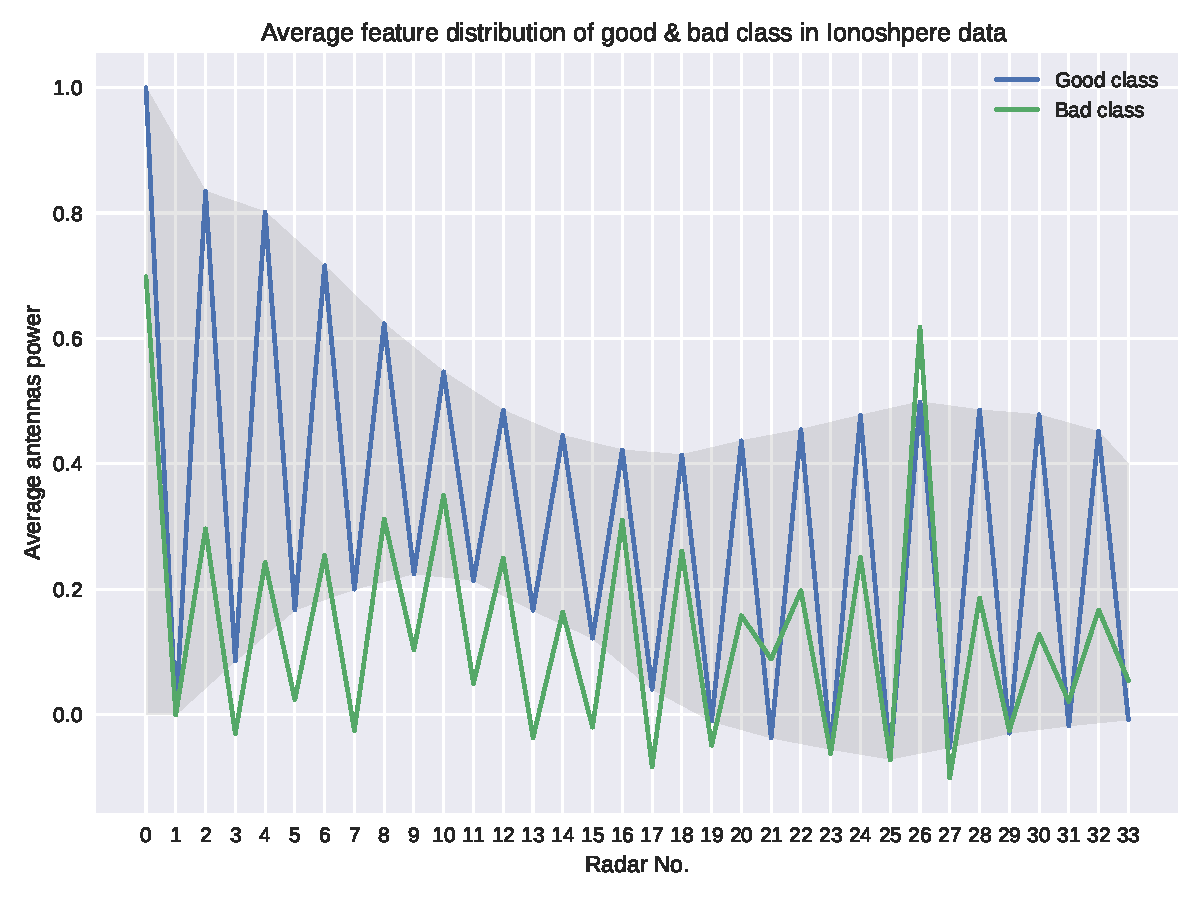
\includegraphics[width=0.7\linewidth]{fig/iono_feat_dist.pdf}
	\caption{Distribution of average numerical features given "good" or "bad" class in ionosphere dataset}
	\label{iono_feat}
\end{figure}

\subsubsection*{Adult Dataset}
Adult dataset aims to predict whether income exceeds \$50K/yr based on census data\cite{kohavi1996scaling}. There are 32561 records and 14 features included with datatypes of continuous count values, continuous real values and categorical/binary values. We min-max normalize the continuous values (both count and real),  discretize normalized real values into 10 categories and leave everything else untouched.


\subsubsection*{Iris Dataset}
There are 4 continuous real value attributes with 1 decimal precision, whose basic statistic information is listed in Figure \ref{iris_des} and Table \ref{iris_table}, where \textit{sl,sw,pw,pw} stand for \textit{sepal length, sepal width, petal width, petal length} \cite{fisher1936use}. Linear correlation between features can be found, e.g. petal length \& petal width and petal length \& sepal length. We also min-max normalize and discretize the normed real values.

\begin{figure}[H]
	\begin{minipage}{0.8\linewidth}
		\begin{minipage}[b]{0.5\linewidth}
		  \centering
		  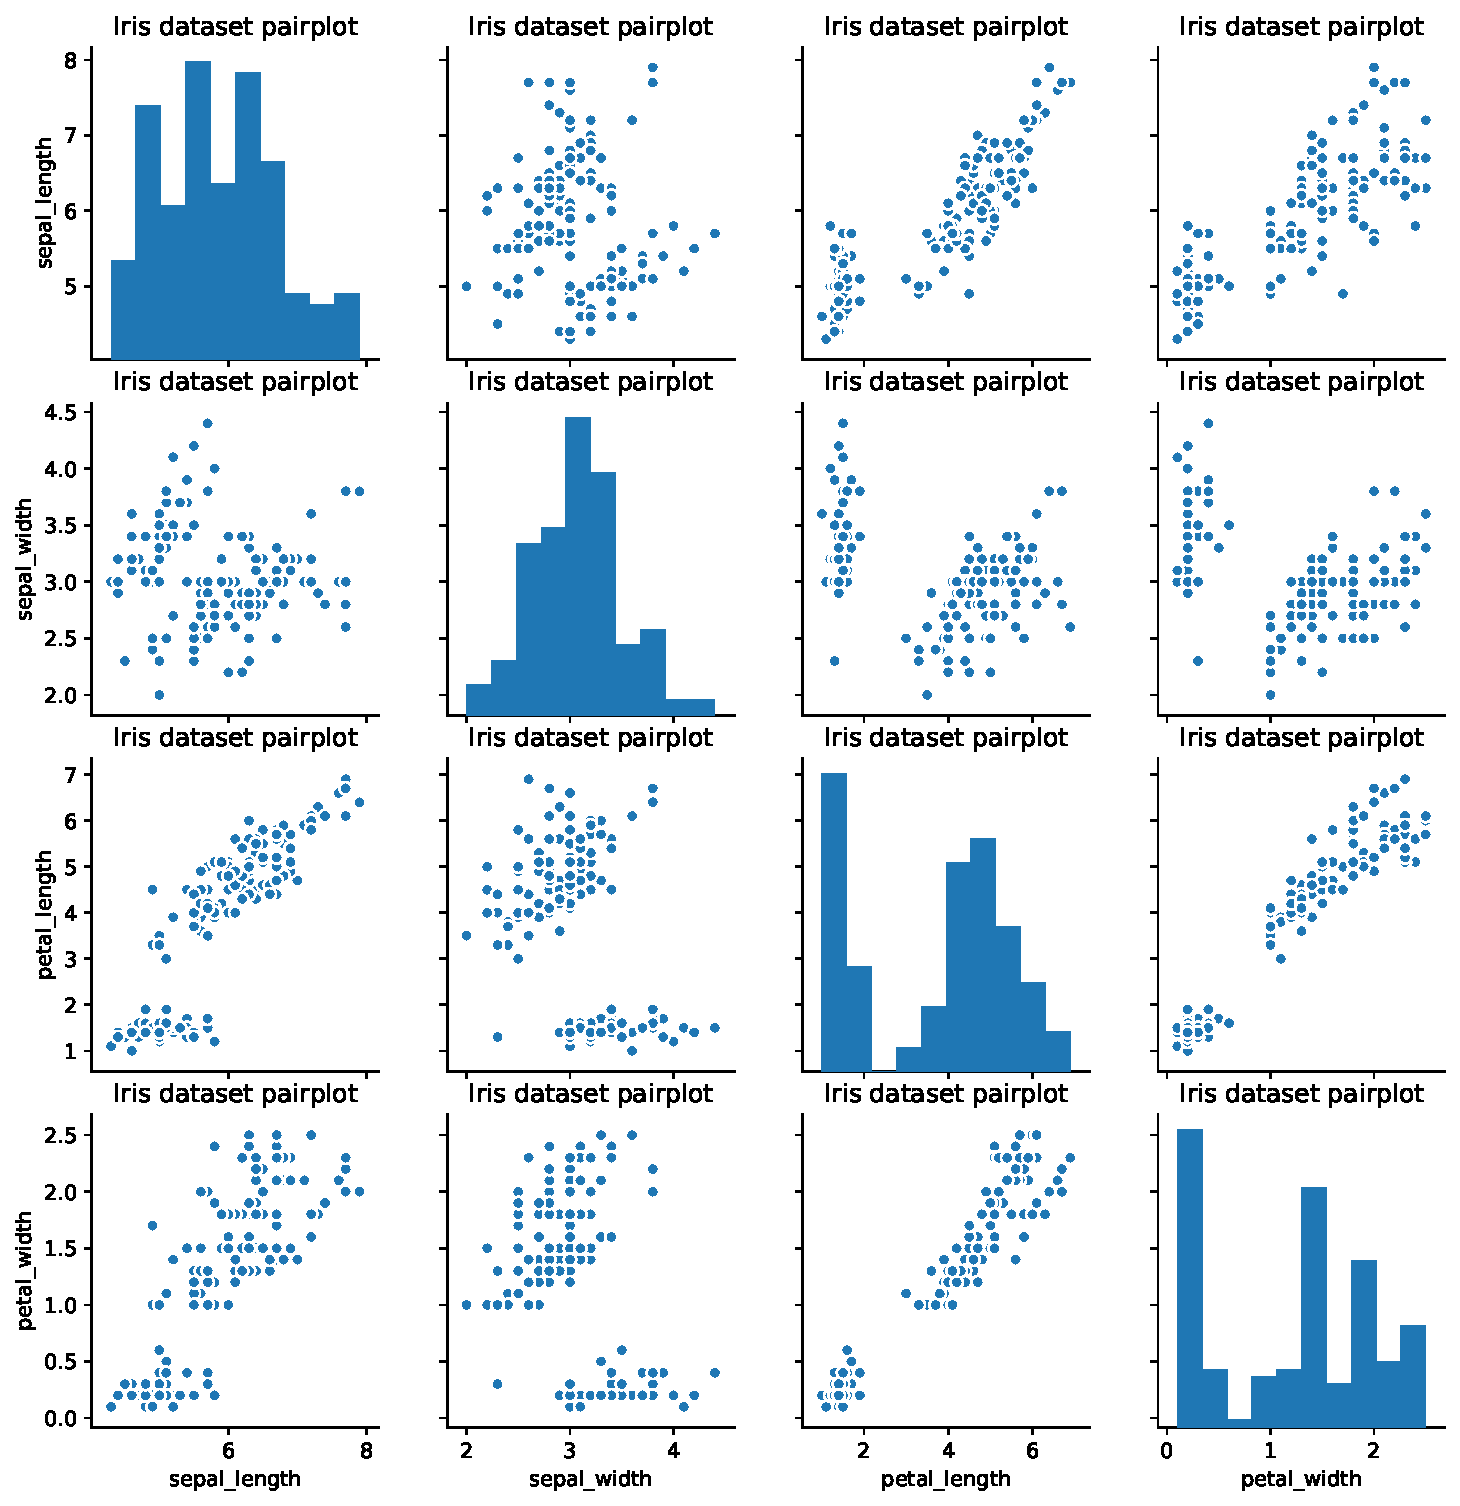
\includegraphics[width= \linewidth]{fig/iris_pairplot.pdf}
		  \captionof{figure}{Pairplot of iris data features}
		  \label{iris_des}
		\end{minipage}
		\hfill
		\begin{minipage}[b]{0.4\linewidth}
		  \centering
			\begin{tabular}{c|cccc}
				\hline
				 & sl & sw & pl & pw \\
				\hline
				count & 150 & 150 & 150 & 150\\
				mean & 5.84 & 3.05 & 3.75 & 1.19\\
				std & 0.82 & 0.43 & 1.76 & 0.76\\
				min & 4.3 & 2.0 & 1.0 & 0.1 \\
				25\% & 5.1 & 2.8 & 1.6 & 0.3\\
				50\% & 5.8 & 3.0 & 4.3 & 1.3\\
				75\% & 6.4 & 3.3 & 5.1 & 1.8 \\
				max & 7.9 & 4.4  & 6.9 & 2.5 \\
				\hline
			\end{tabular} 
		\captionof{table}{Iris data description}
		\label{iris_table}
		\end{minipage}
	\end{minipage}
\end{figure}


\subsubsection*{Car Evaluation Dataset}
In Car Evaluation Dataset, we use 1728 records from 6 categorical features of cars, e.g. price, door number and capacity, to predict the safety level of the cars \cite{bohanec1988knowledge}. This dataset is quite straightforward, we only transform the raw data into categorical features to predict the categorical safety level.


\section{Results}
\subsection*{\underline{Accuracy comparison on four datasets}}

From Table \ref{accuracy_fourdata} , for accuracy of each model, we find that our implemented logistic regression model can work well on small datasets (iris and ionosphere datasets) but worse in larger dataset (car and adult datasets) compared with sklearn model. In the contrary, naive bayes work well on large data set but worse in small dataset.

\begin{table}[H]
	\centering
	\begin{tabular}{c|cccc}
		\hline
		 & iris	 & car & adult & ionosphere \\
		\hline
		logistic regression(ours) &  \textbf{0.75} & 0.65 & 0.66 & \textbf{0.80}\\
		logistic regression(sklearn) & 0.93 & 0.87 & 0.82 & 0.82\\
		naive bayes(ours) & 0.34 &  \textbf{0.69} & \textbf{0.76} & 0.67 \\
		naive bayes(sklearn) & 0.74 & 0.69 & 0.75 & 0.81 \\
		\hline
	\end{tabular} 
	\caption{Accuracy of our implemented model in four datasets comparing to sklearn module}
	\label{accuracy_fourdata}
\end{table}

Furthermore, we compare the different evaluation metrics for binary classification, where ionosphere dataset and adult dataset are selected. Details can be found in Table \ref{binary_comparison}, where \textbf{o} stands for our model and \textbf{s} for results after running \textit{sklearn} module.

\begin{table}[H]

	\begin{tabular}{c|ccccccc}
		\hline
		& &  & ionosphere/adult & dataset & & & \\
		\hline
		& precision(o) & precision(s) & recall(o) & recall(s) & f1(o) & f1(s) & support \\
		\hline
		class 0 &1.00/0.93 &0.90/0.83 &0.48/0.49 &0.48/0.95 &0.65/0.64 &0.86/0.89 &33/4937\\
		class 1 &0.69/0.35 &0.85/0.71 &1.00/0.88 &1.00/0.39 &0.81/0.51&0.88/0.51&37/1575\\
		macro avg &0.84/0.64 &0.88/0.77 &0.74/0.68 &0.74/0.67 &0.73/0.57&0.87/0.70&70/6512\\
		weighted avg &0.83/0.79 &0.87/0.80 &0.76/0.58 &0.76/0.81  &0.74/0.61 &0.87/0.79&70/6512\\

		\hline
	\end{tabular} 
	\caption{Different evaluation metrics of our implemented model in binary-target datasets comparing to sklearn module}
	\label{binary_comparison}
\end{table}

\subsection*{\underline{Learning rate test}}
We mainly test several learning rates with stopping threshold 0.05 in the iris dataset. For small learning rate, such as lr is 0.0001, the accuracy makes no change during the gradient decent, which means that it converges very slow. When the learning rate is very big such as 1 , the accuracy will fluctuate sharply, which means that it will become unstable during gradient descent. We found the best learning rate in our experiment should be around 0.01. so we did hyperparameter search experiment around 0.01, which is in the following figures. We can find the best learning rate for iris should be 0.15, besides we also search the learning rate in ionosphere data set, the best learning rate should be 0.12 according to our experiment.

We have also grid searched for the best stopping thresholds for ionosphere and iris datasets based on the above learning rate tests, which is shown in Figure \ref{stopping_cri_lr}. 

\begin{figure}[htbp]
	\centering
	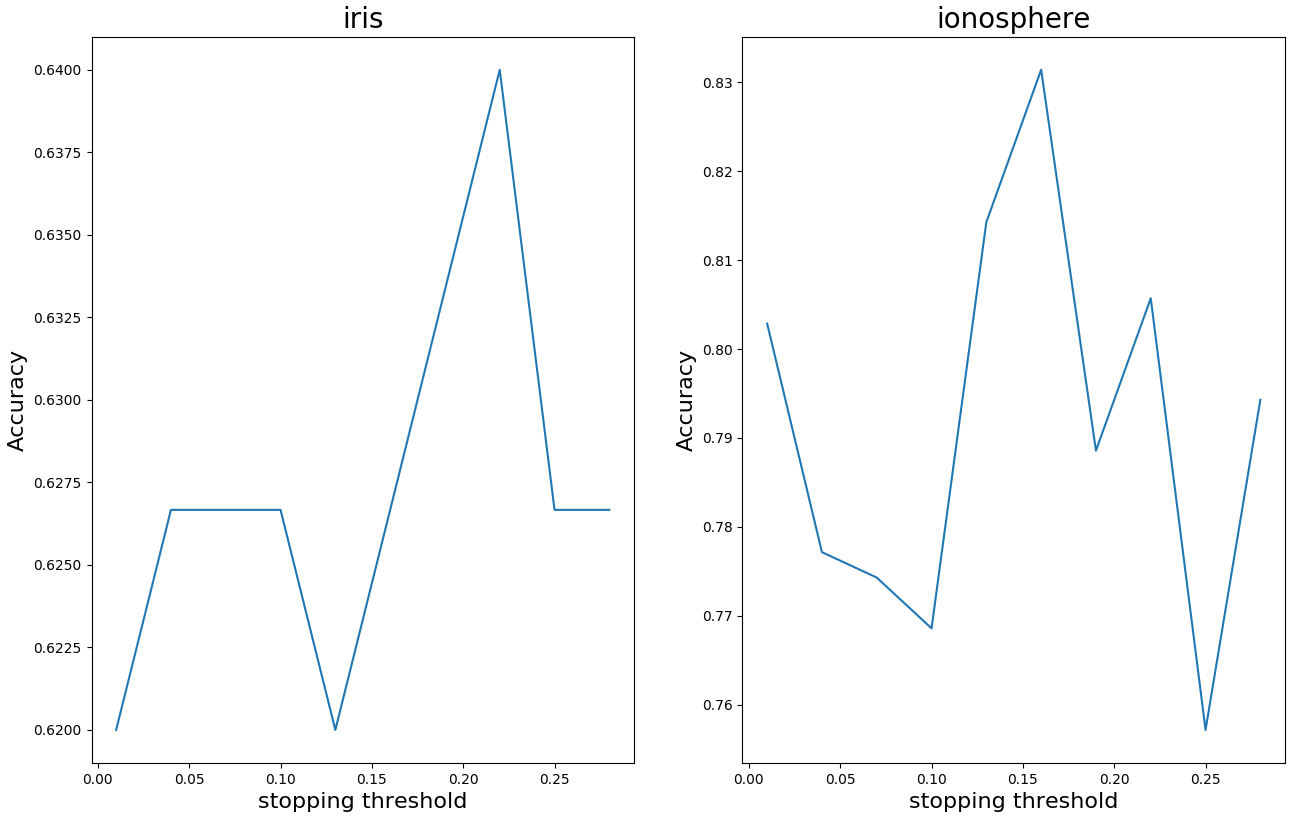
\includegraphics[width=0.8\linewidth]{fig/stopping-threshold.png}
	\caption{Best stopping criterion for Ionosphere Dataset and Iris Dataset given optimal learning rate}
	\label{stopping_cri_lr}
\end{figure}

\subsection*{\underline{Accuracy as a function of the size of dataset}}

From Figure \ref{size_accuracy} we can find that accuracy increases when sample size is roughly less than 200. However, the accuracy becomes stable even the sample size continues growing. 

\begin{figure}[htbp]
	\centering
	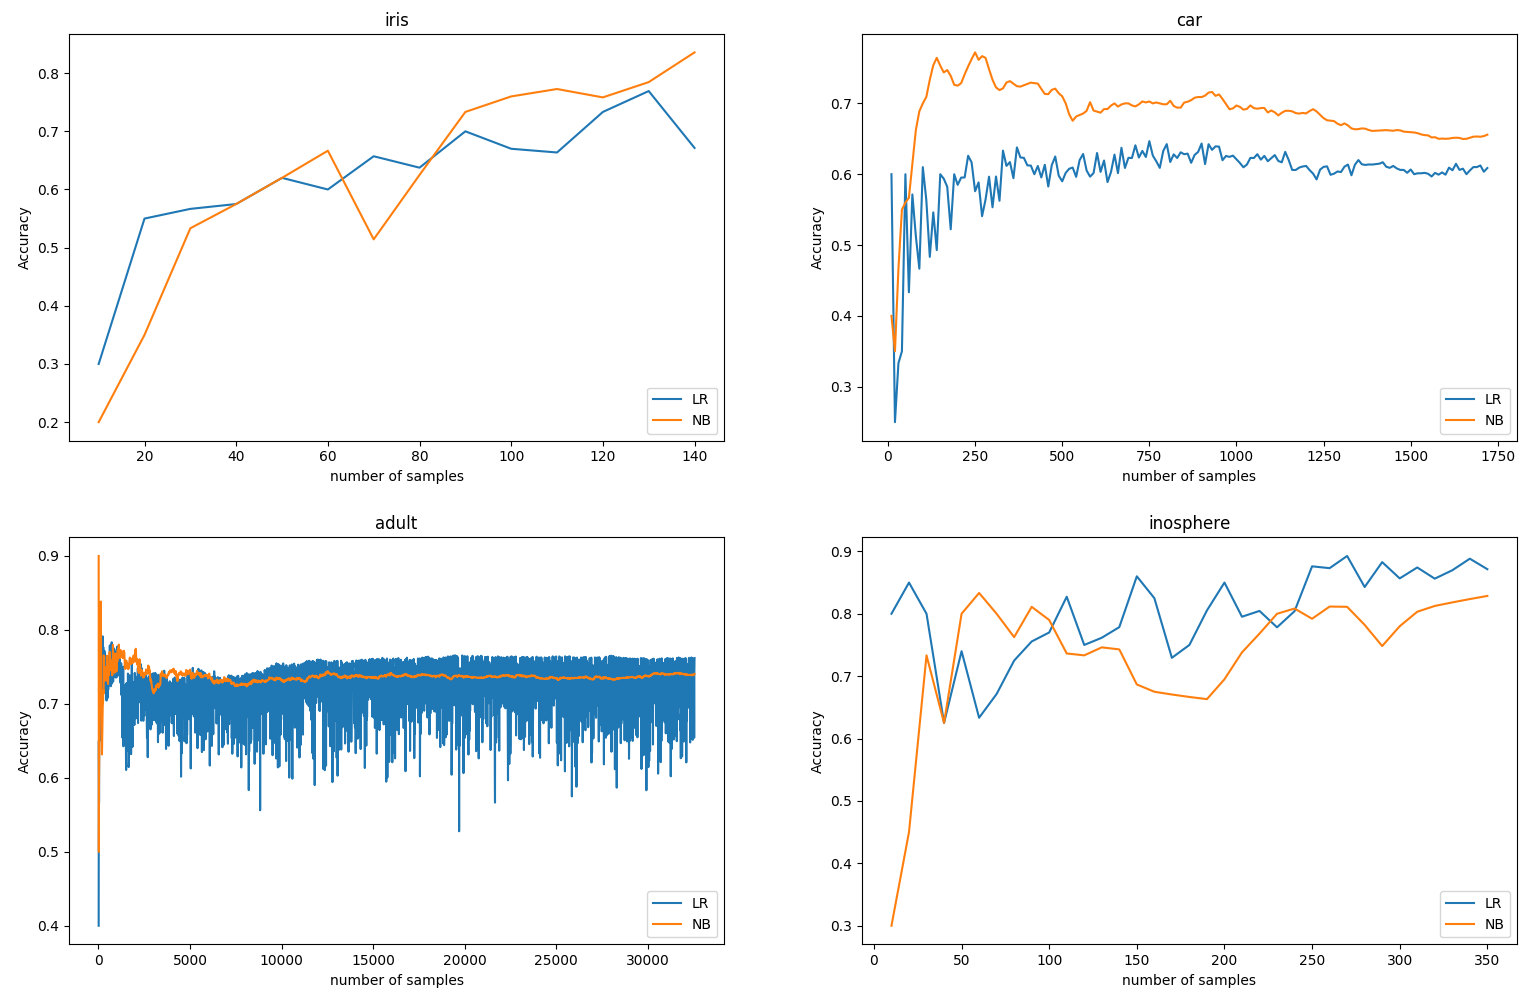
\includegraphics[width=0.8\linewidth]{fig/dataset_size.png}
	\caption{Impact of the training sample size on the accuracy}
	\label{size_accuracy}
\end{figure}


\section{Discussion and Conclusion}

\section{Statement of Contributions}

\begin{itemize}
	\item Dingyi Zhunag: Data preprocessing, data analysis and report formating.
	\item Fuyuan Lyu: Model implementation and report writing.
	\item Tianyu Shi: Running experiment, data visualization and data analysis.
\end{itemize}

\bibliographystyle{unsrt}
\bibliography{a1}

\end{document}
